% Options for packages loaded elsewhere
\PassOptionsToPackage{unicode}{hyperref}
\PassOptionsToPackage{hyphens}{url}
%
\documentclass[
  12pt,
]{article}
\usepackage{amsmath,amssymb}
\usepackage{iftex}
\ifPDFTeX
  \usepackage[T1]{fontenc}
  \usepackage[utf8]{inputenc}
  \usepackage{textcomp} % provide euro and other symbols
\else % if luatex or xetex
  \usepackage{unicode-math} % this also loads fontspec
  \defaultfontfeatures{Scale=MatchLowercase}
  \defaultfontfeatures[\rmfamily]{Ligatures=TeX,Scale=1}
\fi
\usepackage{lmodern}
\ifPDFTeX\else
  % xetex/luatex font selection
\fi
% Use upquote if available, for straight quotes in verbatim environments
\IfFileExists{upquote.sty}{\usepackage{upquote}}{}
\IfFileExists{microtype.sty}{% use microtype if available
  \usepackage[]{microtype}
  \UseMicrotypeSet[protrusion]{basicmath} % disable protrusion for tt fonts
}{}
\makeatletter
\@ifundefined{KOMAClassName}{% if non-KOMA class
  \IfFileExists{parskip.sty}{%
    \usepackage{parskip}
  }{% else
    \setlength{\parindent}{0pt}
    \setlength{\parskip}{6pt plus 2pt minus 1pt}}
}{% if KOMA class
  \KOMAoptions{parskip=half}}
\makeatother
\usepackage{xcolor}
\usepackage[left = 2.54cm, right = 2.54cm, top = 2.54cm, bottom =
2.54cm]{geometry}
\usepackage{graphicx}
\makeatletter
\def\maxwidth{\ifdim\Gin@nat@width>\linewidth\linewidth\else\Gin@nat@width\fi}
\def\maxheight{\ifdim\Gin@nat@height>\textheight\textheight\else\Gin@nat@height\fi}
\makeatother
% Scale images if necessary, so that they will not overflow the page
% margins by default, and it is still possible to overwrite the defaults
% using explicit options in \includegraphics[width, height, ...]{}
\setkeys{Gin}{width=\maxwidth,height=\maxheight,keepaspectratio}
% Set default figure placement to htbp
\makeatletter
\def\fps@figure{htbp}
\makeatother
\setlength{\emergencystretch}{3em} % prevent overfull lines
\providecommand{\tightlist}{%
  \setlength{\itemsep}{0pt}\setlength{\parskip}{0pt}}
\setcounter{secnumdepth}{5}
\usepackage{float}
\usepackage{sectsty}
\usepackage{paralist}
\usepackage{setspace}
\setstretch{2.0}
\usepackage{fancyhdr}
\usepackage{ragged2e}
\usepackage{lastpage}
\usepackage{dcolumn}
\usepackage{natbib}\bibliographystyle{agsm}
\usepackage[nottoc, numbib]{tocbibind}
\ifLuaTeX
  \usepackage{selnolig}  % disable illegal ligatures
\fi
\usepackage{bookmark}
\IfFileExists{xurl.sty}{\usepackage{xurl}}{} % add URL line breaks if available
\urlstyle{same}
\hypersetup{
  hidelinks,
  pdfcreator={LaTeX via pandoc}}

\title{\textbf{Examining The Effect of Padding on Facial Recognition Using Convolution Neural Networks}}
\author{}
\date{\vspace{-2.5em}}

\begin{document}
\maketitle

\allsectionsfont{\centering}
\subsectionfont{\raggedright}
\subsubsectionfont{\raggedright}

\pagenumbering{gobble}

\begin{centering}



\includegraphics[width=0.8\linewidth]{img/jkuatlogo} 
\vspace{0.3cm}

\large
Wycliffe Atswenje Sikolia \vspace{0.3cm}

A Research Proposal Submitted in Partial Fulfillment of The Requirements for The Award of a Post Graduate Diploma in Applied Statistics of Jomo Kenyatta University of Agriculture and Technology.\vspace{1cm}

2024 

\end{centering}

\newpage

\pagenumbering{roman}

\begin{centering}

{\bf DECLARATION}

\end{centering}

\normalsize

This research proposal is my own work and has not been presented
elsewhere for a degree award.

Signature
\ldots\ldots\ldots\ldots\ldots\ldots\ldots\ldots\ldots\ldots\ldots\ldots\ldots.
Date \ldots\ldots\ldots\ldots\ldots\ldots\ldots\ldots..

Wycliffe Atswenje Sikolia

SCB384-3284/2013

\textbf{Declaration by supervisors}

This research proposal has been submitted for examination with our
approval as university supervisors.

Signature
\ldots\ldots\ldots\ldots\ldots\ldots\ldots\ldots\ldots\ldots\ldots\ldots\ldots.
Date \ldots\ldots\ldots\ldots\ldots\ldots\ldots\ldots..

Dr.~Anthony Kibira Wanjoya

Department of Statistics and Actuarial Sciences

Jomo Kenyatta University of Agriculture and Technology

Signature
\ldots\ldots\ldots\ldots\ldots\ldots\ldots\ldots\ldots\ldots\ldots\ldots\ldots.
Date \ldots\ldots\ldots\ldots\ldots\ldots\ldots\ldots..

Dr.~Jane Aduda

Department of Statistics and Actuarial Sciences

Jomo Kenyatta University of Agriculture and Technology

\newpage

\begin{centering}

{\bf DEDICATION}

\end{centering}
\large

To my Family and Friends.

\newpage

\begin{centering}

{\bf ACKNOWLEDGEMENT}

\end{centering}
\large

Special regards to my supervisors Dr.~Anthony Kibira Wanjoya and
Dr.~Jane Aduda for their guidance and relentless criticism on this work.
Their continuous support, insightful comments, and demand for excellence
have played a crucial role in this work. I am particularly grateful to
my father whose moral support has been instrumental in my studies. My
friends and family have also helped during the course of my studies by
reminding me of the need to focus and complete my studies, which is the
reason I got this far. Their words of positive affirmation gave me a
shoulder to lean on when the going got difficult. I would also like to
thank members of the department of statistics and actuarial sciences
from the Jomo Kenyatta University of Agriculture and Technology for
their support in my studies. Most importantly I would like to thank the
almighty God for granting me the knowledge to carry out this study

\newpage

\begin{centering}

{\bf ABSTRACT}

\end{centering}

\doublespacing
\large

Facial recognition technology is the development of solutions that can
match a face from an image or a real time video to that of a known
person. While such technology exists, no research has been done to
examine the effect of padding on facial recognition. This study aims to
contribute to the existing literature by developing a facial recognition
solution by comparing the effect of padding using a self-built model and
a pre-trained model. It follows that the study will add value to the
existing knowledge by creating a guideline that could be used when there
is need to make a decision between creating an accurate model and saving
on the training time.

\newpage

\centering
\raggedright
\newpage

\tableofcontents

\newpage

\begin{centering}

{\bf List of Tables}

\end{centering}

\doublespacing
\large

\newpage
\listoffigures

\doublespacing
\large

\newpage

\begin{centering}

{\bf List of Abbreviations and Acronyms}

\end{centering}

\doublespacing
\large

\newpage
\pagenumbering{arabic}

\doublespacing
\large
\justifying

\section{Chapter One}\label{chapter-one}

\section*{Introduction}\label{introduction}
\addcontentsline{toc}{section}{Introduction}

\subsection{Background of Study}\label{background-of-study}

~~~~~~~The ability of workers to consume technology and adapt to
emerging technology is quickly influencing the job market. The World
Economic Forum (2023) estimates that by 2027, task automation in the
global job market is likely to vary from 35\% reasoning and
decision-making to 65\% information and processing by 2027. This is a
clear indicator that data scientists are marketable. In a different
publication, Vicario and Coleman (2018) mention that data scientists
work in industries such as technology, production industries,
e-commerce, and even agriculture. Clearly, the need for skilled
personnel in data science is growing at an alarming rate, which has
resulted in a lot of competition among giant companies in technology.
This has led to innovations such as speech recognition (Siri) by apple,
image detection by Google, and video recommendation from YouTube.
Indeed, giant technology companies are consuming big data to create
applications that are revolutionizing the world. These recent
innovations prove that data science is growing rapidly and that the
world is yet to see additional applications that will consume big data.

~~~~~~~The big data era is fueled by gadgets that emit and store huge
amounts of data. Examples of such gadgets include the smartphones,
laptops, desktops, and IOT devices such as smart watches, and smart
refrigerators. Owing to the recent increase in the amount of such data,
people today store their extra data in the cloud and external hard
drives but some people still store their data in gadgets that produce
that data. Critical to the discussion is the fact that smartphones have
limited storage spaces implying that smartphone users at times extend
their storage to the cloud. Additionally, the huge amount of storage
space in smartphones is consumed by images and videos. These images and
videos are mostly from social media while some of them come from
pictures and videos recorded from smartphones. In short, smartphones
produce a considerable amount of data that should be harnessed to make
the world a better place.

~~~~~~~Indeed, huge technology companies such as Google and Apple have
developed world class applications that have enabled them to enjoy a
competitive advantage over other companies.These data science
applications (from Google and Apple) have been made possible by
techniques such as support vector machines, random forests, decision
trees, and neural networks. The term neural network refers to a
connection of layers composed of units called perceptrons, which is made
up of an input layer (the predictor variables), a processing unit, and
an output layer (the response variable). The processing unit could
comprise one or more hidden layers. That said, deep learning occurs when
a neural network is created with more than one hidden layer. Having
defined deep learning, it is imperative to highlight that decision trees
and support vector machines were more famous than neural networks.
However, the neural networks were brought to fame when Geoffrey Hinton
et al., (2006) developed a neural network that predicted handwritten
digits with an accuracy of 98\%.

~~~~~~~Another field that emerged from deep learning is facial
recognition. Lately, the field of facial recognition has attracted a lot
of attention from scholars and practitioners. Some of the innovations
that have emerged from facial recognition include development of home
authentication systems, attendance management systems, security
surveillance systems, and emotion recognition systems. Critical to the
debate is the fact that different solutions of creating facial
recognition systems have been proposed. One of the techniques that is
used for facial recognition is convolution neural networks, which relies
on hyper parameters like pooling, padding, strides, kernels, and the
activation function. All these parameters affect the output of
convolution neural networks differently. This is a clear indicator that
studies examining how the mentioned hyper parameters affect the
performance of convolution neural networks need to be discussed with an
aim of developing a road map that could be used to train convolution
neural networks.

\subsection{Statement of the Problem}\label{statement-of-the-problem}

~~~~~~~Researchers in facial recognition have developed solutions such
as FaceNet, VGGFACE, VGG16, VGG19, OpenFace, and DeepFace. Even though
existing solutions on facial recognition have been developed, the number
of publications that investigate the effect of hyper parameter tuning on
facial recognition are few. The publications become even fewer when the
problem is narrowed down to convolution neural networks. Examples of
hyper parameters that could be investigated under neural networks
include padding, strides, filters, pooling, kernel size, the batch size,
the learning rate and the number of layers. Critical to the debate is
the fact that same padding, valid padding, causal padding and constant
padding are some of the padding techniques used in deep learning. The
most famous types of padding are valid and same padding. This begs the
question: What would come out of examining the effect of padding on
facial recognition? It is why this study aims to examine the effect of
padding on facial recognition using data collected from smartphone
images at Samasource.

\subsection{Justification of the
study}\label{justification-of-the-study}

~~~~~~~The justification of this study relies on the fact that
convolution neural networks is the one stop shop when developing
solutions in computer vision. Here, the term computer vision is defined
as a facet in deep learning that develops solutions by analyzing images
or videos. One of the important hyper parameters used in convolution
neural networks is padding. Padding could be elucidated as a technique
used to add data to an image's borders, which results in the increase of
the image's height, width or depth. It is important to note that padding
adds value in the training process of convolution because it could be
used for dimension preservation or maintaining border information.
Indeed, padding is an important hyper parameter used in training
convolution neural networks because of the value it adds in the
performance of a convolution neural network.

~~~~~~~Given the role padding plays in training convolution neural
networks, it is important to examine how different padding methods
contribute to the performance of a convolution neural network. This owes
to the reality it would help scholars and practitioners implement the
right padding technique for the right problem. Moreover, it would be
prudent to tell how padding affects the accuracy and training time of a
model. This will help practitioners and scholars when making decisions
that rely on the accuracy and training time of facial recognition
models. Simply put, this publication will enable researchers to choose
whether or not to implement padding when the training time of a model is
of the essence. Likewise, it will aid scholars to make the decision of
whether or not to implement padding when the accuracy of a facial
recognition is the main goal of building the model.

\subsection{OBJECTIVES}\label{objectives}

\subsubsection{General Objectives}\label{general-objectives}

To examine the effect of padding on facial recognition using convolution
neural networks and data collected using a smartphone.

\paragraph{Specific Objectives}\label{specific-objectives}

\begin{enumerate}
\def\labelenumi{\arabic{enumi}.}
\tightlist
\item
  To build a facial recognition model using convolution neural networks
\item
  To examine the effect of padding on a pre-trained model: VGGFACE-16.
\item
  To examine the effect of padding on facial recognition using a
  self-trained model
\item
  To compare the effect of padding on VGGFACE-16 and a self-built model.
\end{enumerate}

\newpage
\doublespacing
\large
\justifying

\section{Chapter Two}\label{chapter-two}

\section*{Literature Review}\label{literature-review}
\addcontentsline{toc}{section}{Literature Review}

\subsection{Introduction}\label{introduction-1}

~~~~~~~This section surveys previous works done on facial recognition
with a bias towards the objectives of this work. It begins with
examining different types of methodologies that have been used for
facial recognition before delving into how different types of neural
networks have been used for facial recognition. Specifically, this
proposal discusses how convolution neural networks, artificial neural
networks, and how they have been used for facial recognition. It also
discusses padding and how they can be applied to convolution neural
networks mentioning different types of padding strategies. It is then
that the paper examines and discusses different datasets used in facial
recognition before discussing three facial recognition architectures
that have been used in facial recognition.

\subsection{Facial Recognition}\label{facial-recognition}

~~~~~~~Facial recognition is a biometric technique used to identify
faces and match those faces to a database of faces with an aim of
identifying a human being from an image. From the definition, it is
clear that face recognition is a two-step process with the first step
being face detection and the second step being face identification. The
first step of facial recognition (or the face detection step) is
identifying and extracting human faces from an image. In this step, all
objects in an image are extracted and checked to confirm if a picture
contains a human face. If any human face is present in the image, the
face is extracted from the image before step two begins. In the second
step or the image identification step, an image is compared to faces
stored in a database to identify if the face matches the face of a known
person. In short, there is a difference between facial detection and
facial recognition and that facial recognition begins with facial
detection and finalizes with facial identification.

\subsubsection{Face Detection}\label{face-detection}

~~~~~~~Given an arbitrary image, the objective of facial detection is to
establish whether or not there are any faces in the image and if
present, return the image location and extent of each face (Yang et al.,
2002). It is important to highlight that there are several methods that
could be used for detecting faces from images. These methods include
knowledge based methods, feature invariant approaches, template matching
methods, and appearance based methods. Indeed, the mentioned methods are
important when detecting faces from images, but all these methods are
accompanied by several challenges. This owes to the reality that Yang et
al., (2002) list the following five challenges that are associated with
facial detection: - pose, occlusion, aging face expression, imaging
conditions and image orientation. Moreover, face expression is not only
a challenge in face detection but also in face recognition. It follows
that researchers on facial recognition should identify methods of
tackling the mentioned challenges associated with face detection.

\paragraph{\texorpdfstring{Challenges in Face Detection\\
}{Challenges in Face Detection }}\label{challenges-in-face-detection}

\textbf{Pose}: A review of images databases will indicate that people
like taking images in different poses. It follows that an image is
likely to have a face that is twisted to the right, left, or even upside
down. Moreover, some features such as the nose, eye, or ears maybe
wholly or partially occluded which is an additional challenge in facial
recognition. This problem is always solved by rotating images back to an
upright position.

\textbf{Occlusion}: Human beings often have features that could affect
image detection. For instance, men are known to have beards, which may
or may not exist in images. It is also important to highlight that
people at times wear spectacles, which also affects face detection.
Moreover, COVID 19 forced people to wear masks, which present a unique
challenge in facial recognition.

\textbf{Aging}: Human faces are known to change with age progression
which presents a challenge in facial recognition. This implies that
there would be a significant difference in images if the time difference
between the images is large. It is notable that aging will not be a
challenge to this paper because people tend to change their smartphones
for a few years. It is notable however that Singh and Prasad (2018)
propose the use of coupled auto-encoder networks and non-linear analysis
as a solution to the aging problem in facial recognition.

\textbf{Facial expressions}: Images of human faces could also be
affected by their emotions because people can change their faces based
on emotions they are experiencing. Critical to the discussion is the
reality that Singh and Prasad (2018) cite expression invariant 3D face
recognition as a solution to the problems of facial expressions in image
recognition. Imaging conditions and image orientation: A huge chunk of
solutions in computer vision make the assumption that there is a single
illuminant lighting in an image. Regardless, that is not always the
case. As evidenced, Finlayson and Fredembach (2007) reveal that images
always contain shadows depending on the positions from different lights
that affect an image. Important to the debate is the truth that
Finlayson (2018) proposes a solution to the problems arising from
illumination in computer vision.

\paragraph{\texorpdfstring{Face Detection Approaches\\
}{Face Detection Approaches }}\label{face-detection-approaches}

\textbf{Knowledge Based Methods of Facial Detection}\\
\vspace{-2.8em}

~~~~~~~This method relies on a set of rules to detect whether there is a
human face in an image. The method captures the human knowledge of faces
and interprets the knowledge into a set of rules. For instance, the face
has two symmetric eyes; the eye areas are darker than the cheeks, the
distance between eyes, and the difference in colors between the eyes and
cheeks. It is notable that using the knowledge base method for face
detection could be difficult because it is difficult to develop a set of
rules that can correctly identify a human face. This owes to the fact
that there could be very many false positives if the rules are too
general. Likewise, there could be many false negatives if the rules are
too strict. This drawback has hampered researchers from using this
technique. However, Chen et al., (2001) used the knowledge based method
to detect faces in an image with an accuracy of 94\%. One disadvantage
with this method is that it is not efficient.

\textbf{The Feature Invariant Approach of Face Detection}\\
\vspace{-2.8em}

~~~~~~~The feature invariant method of face detection is a little bit
different from the knowedge based method because it uses statistical
methods on facial landmarks. Celiktutan et al, (2013) define a face
landmark as a prominent feature that can play a discriminative role or
can serve as anchor points in face detection. Examples of such landmarks
include the eye corners, the nose tip, nostril corners, mouth corners,
end points of eyebrow arcs, ear lobes, and the chin. This approach works
by detecting facial landmarks, texture and skin color before using a
statistical model to identify the presence of a face in an image.
Critical to the discussion is the reality that different authors have
used the feature invariant approach for face detection. For instance,
Kapil and Jain (2013) compared texture based to the structure and shape
based feature invariant based methods and concluded that the texture
based method is more accurate. However, the authors argue that feature
invariant based methods are computationally expensive.

\textbf{The Template Based Approach of Face Detection}\\
\vspace{-2.8em}

~~~~~~~This method functions to extract facial image features to gain
the Euclidean distance value served as input face comparison value of
the users' faces stored in the database (Hidayat, Wibowo, Satria,
Winursito, 2021). Simply put, the template based approach transforms an
image into geometric primitives like curves and points. This is done by
identifying distinctive features like the eye, the nose, the chin, and
the mouth before measuring their relative positions, widths and other
parameters of the distinctive features. Features extracted from an image
are then compared to known features of a human face to check whether an
image is that of a human face. For further elucidation the eye, nose,
mouth and the chin are compared to that of a human face. If the features
obtained from the image match those of a human face, then the object in
question is declared to be a human face. It is vital to note that
Hidayat, et al., (2021) assert that the template approach of facial
recognition is known to have a lighter computational load than other
methods because it does not require features from the entire face.

\textbf{The Appearance Based Approach of Facial Detection}\\
\vspace{-2.8em}

~~~~~~~The idea behind using Appearance methods for face detection
relies on the linear algebra concept of subspaces. This approach of
facial detection relies on the entire face, which is taken in as an
input image data. The data collected from the input image is processed
into a two dimensional pattern that is later used to decide whether
there is a human face in an image. Critical to the discussion is the
fact that this technique finds the best facial features because it
rejects redundant information and keeps important information. Vital to
the discussion is the fact that different authors have used the
appearance based technique successfully. For example, Rusia and Singh
(2023) used the appearance based technique of facial recognition and
examined some of the face identity threats faced by this technique.
Regardless, Yan et al., (2018) argues that appearance based methods are
computationally expensive and have difficulty handling substantial
amounts of facial variations.

\subsubsection{Face Identification
Approaches}\label{face-identification-approaches}

~~~~~~~As already mentioned, facial recognition is a two-step process
with the first face being the face detection and the second step being
the face identification step. The face identification phase is where
facial characteristics are extracted from a detected face and compared
to a known face to confirm if the facial characteristics match those of
the known face. Evidence from literature suggests that the template
approach and the appearance based approaches are not only used in face
detection but could also be used in face identification. As evidenced,
Proyecto (2010) discusses template matching and the appearance based
technique in both face detection and face identification. It is
important to highlight that different publications on techniques that
are used in face identification exist. Apart from template matching and
appearance based methods, statistical approaches are also used in face
identification.

\paragraph{\texorpdfstring{Template Matching / Geometric Approaches\\
}{Template Matching / Geometric Approaches }}\label{template-matching-geometric-approaches}

~~~~~~~The template matching or the geometric approach of facial
recognition is similar to the template matching of the face detection
step. However, the objective of the facial recognition step is different
from the objective in the face identification step. This owes to the
reality that the objective of the facial recognition step is to match a
face to a known person while the objective in the face detection step is
to identify whether an object in an image is a human face or not. Like
in the face detection step, features like the eye, the nose, the chin,
and the mouth are extracted from a human face before matching the
features in question to a known face. Consider a face A belonging to a
person B and a face C belonging to an unknown person. The template
matching approach will collect facial characteristics from faces A and
C. These characteristics from the unknown face C will be compared to
characteristics from the known face A. If a match is found, then the
decision will be that the unknown face C belongs to person B.

~~~~~~~It is critical that several authors have applied the geometric
approach of facial recognition in their studies. For example, Ghimire
and Lee (2016) used the approach in question to predict emotions on a
sequence of images that were extracted from videos. Specifically,
Ghimire and Lee (2016) ran a multi-class AdaBoost algorithm and a
support vector machines algorithm on the Cohn-Kanade (CK+) facial
expression database and obtained an accuracy of 95.17\% and 97.35\%
respectively. Another example of a study that used the geometric
technique of facial recognition is one by Ayo et al., (2021). This owes
to the reality that the authors in question used the geometric approach
of facial recognition together with the you-only-look-once (YOLO)
algorithm to predict age, gender and emotions. In their study, the
authors were able to predict gender and emotions with an 80\% accuracy.
Regardless, Ayo et al., (2021) were not able to predict age accurately
and mentioned that accurate age prediction was hampered by the lighting
conditions of a face.

\paragraph{\texorpdfstring{Appearance Based Methods\\
}{Appearance Based Methods }}\label{appearance-based-methods}

~~~~~~~Appearance based methods of face identification work the same way
they work for face detection with the difference being the purpose of
the method. This owes to the fact that the entire face is used to
identify a face but with an aim of matching a face to that of a known
person. It is important to highlight that this technique could be
classified into linear and non-linear methods. Examples of linear
methods include principal components analysis, independent component
analysis, linear discriminant analysis, and linear regression
classifier. Non-linear methods include kernel principal component
analysis, local linear embedding, and kernel linear discriminant
analysis. In a nonlinear approach the input image is mapped into higher
dimensional space in which the face is simplified and linear. In
principal component analysis a number of images are taken using gray
levels. Each image is mapped to a long vector of gray levels. Several
views of each person are collected in the database during training.
During recognition a vector corresponding to an unknown face is compared
with all vectors in the database (Viegas et al., 2019).

~~~~~~~It is imperative to mention that several authors have
investigated the appearance based method for facial recognition. For
instance, Struc and Pavesic (2009) examine the performance of appearance
based methods subject to different environmental factors and conclude
that the linear discriminant analysis produces the best results across
different environmental conditions. Wu et al., (2018) also debate
appearance based methods of facial recognition by examining facial
expressions using the technique in question. The authors controlled for
lighting conditions using a histogram equalization technique and a
brightness preserving technique and concluded that the brightness
preserving technique performs better than the histogram equalization
technique. Broti (2019) also examines appearance based methods of facial
recognition by discussing the principal components analysis, independent
component analysis, linear discriminant analysis methods used in facial
recognition. A drawback for this method is that it is challenging to
find an efficient combination of dimensionality reduction technique and
classifier.

\subsection{Types of Neural Networks}\label{types-of-neural-networks}

~~~~~~~The single layer neural network architecture is the basis of
neural networks and has already been discussed in the introductory
section of neural networks. Other types of neural networks include the
multiple layer neural networks, radial basis functions neural networks,
restricted Boltzmann machines, the convolution neural network, and the
recurrent neural network. However, the multilayer neural network (ANN),
and the convolution neural network will be discussed in this paper
because those are some of the tools the researcher will be using in this
study.

\subsubsection{Multiple Layer Neural
Network}\label{multiple-layer-neural-network}

~~~~~~~As the title immediately above suggests a multilayer neural layer
architecture is formulated when two or more networks are used to develop
a neural network. A multilayer neural network consists of an input
layer, which feeds in data to the first layer of the neural network. The
first layer then feeds in data to at least one additional layer before
sending the results to an output layer (for a case of a neural network
with two layers). It is important to highlight that the training process
of a multilayer neural network (also called artificial neural networks)
involves the backpropagation algorithm or the generalized Delta rule (Da
Silva et al., 2017). The backpropagation algorithm is best described as
follows: The multilayer neural network begins by setting random weights
during the first pass across the neurons. Upon reaching the output of
the neuron, the weights are compared to the actual output and readjusted
accordingly until the predicted value of the neuron is close to the
actual value.

~~~~~~~Artificial neural networks have been used for facial recognition
widely. For example, Zhang et al., (2022) applied the artificial neural
network algorithm on facial biological image information recognition and
scanning. Specifically, the authors involved a methodology that used
imaging technology to detect and extract the biological attributes of
the image. In a different publication, Wang et al., (2021) conducted a
study with an aim to examine the problem of identifying human faces
given different and complex backgrounds. Specifically, the authors used
neuron regenisis mechanism and the synapse mechanism to identify facial
images from complex backgrounds. The scholars in question developed a
model called Where-What Networks that is able to learn type, location
and size, which is able to identify human faces from complex
backgrounds. This is a clear indicator that researchers are using
artificial neural networks for facial recognition and that much is yet
to be seen on facial recognition.

~~~~~~~Evidence from examining different publications on artificial
indicates that they are being used for facial recognition. Regardless,
artificial neural networks (ANN) are known to have their limitations.
For example, Balarini et al., (2011) assert that ANNs require a lot of
time to train a model. The problem becomes even worse if the number of
neurons and hidden layers required to train a model is high. This
problem is controversial because neural networks are known to register a
high accuracy when a high number of neurons and hidden layers are used.
Every neuron in each layer can make calculations independent of other
neurons implying that graphics processing units could help solve the
time problem required to train an ANN model. Another problem associated
with ANNs is the vanishing gradient problem. Tarnate et al., (2020)
define the vanishing gradient problem as a case when the neural network
becomes too deep hence the network becomes hard to train and could
result in a situation where network will not finish its training
process.

~~~~~~~It is evident that ANNs have their disadvantages, but that does
not mean that there are no advantages of using them. For example, Roza
and Mohsen (2021) discuss some of the advantages of ANNS arguing that
they have an extraordinary ability of in learning well in the face of
minor disturbances. In simple terms, ANNs are fault tolerant because a
disturbance in one of the neurons will not prevent the entire network
from generating an output. Another advantage of ANNs is the fact that
they can learn and model non-linear and complicated interactions. This
is crucial because many of the relationships between inputs and outputs
in real-life situations are non-linear and complex. It is also notable
that while the process of training ANNS takes time, they become
efficient in the end because it would take a shorter time than creating
a set of instructions using traditional programming.

\subsubsection{Convolution Neural
Networks}\label{convolution-neural-networks}

~~~~~~~A Convolution neural network (CNN) is a type of artificial neural
network that has one or more convolution layers and are used mainly for
image processing, classification, and segmentation. CNNs are similar to
ANNs described above only that they assume that the input is an image
like dataset. Consequently, CNNs use a convolution layer, a pooling
layer, a fully connected layer and an activation function layer, which
makes them different from ANNs. Koodalsamy, et al., (2023) have a
publication that discusses the layers used in convolution neural
networks. Specifically, the convolution layer is where an image is
subjected to a set of filters; the pooling layer is where the
dimensionality of an image is reduced; the fully connected layer is
where the output of the pooling layer is flattened; and the activation
function is where a decision is made. A thorough discussion of all these
layers will be discussed in the methodology section of this paper.

~~~~~~~Like artificial neural networks, convolution neural networks have
been used for facial recognition widely. For example, Xiaobo et al.,
(2023) recognize that facial recognition is hampered by factors such as
posture, light and the background of the image. As a result, the authors
proposed the addition of an attention mechanism to convolution neural
networks in a bid to reduce the effects of factors that affect facial
recognition. In a different paper, He et al., (2023) recognize that the
existing methods on facial recognition ignore the effect of spatial
relationships between predictors. Consequently, the authors introduced
the use of a Group Depth-Wise Transpose Attention (GDTA) block, which is
designed to establish long range dependencies in different facial
features. This led to the development of a lightweight face recognition
model, which the authors call CFormerFaceNet. Shalini et al., (2023)
also did some work on facial recognition using CNNS by proposing the use
of CNNs for creating attendance management systems that could be used
for monitoring students' classroom attendance.

~~~~~~~It is important to highlight that CNNs have advantages that makes
them suitable for deep learning. As evidence of this, Zhang et al.,
(2018) discusses some of the advantages of using convolutional neural
networks. According to the authors, CNNs bypass the feature engineering
stage of deep learning because feature engineering in CNNs is done
during the training time. Another advantage of convolution neural
networks is that they allow weight sharing, which in turn improves the
efficiency of CNNs. Critical to the discussion is the fact that weight
sharing is a wide topic that has been discussed by several authors
including Dupuis et al., (2021) and cannot be discussed exhaustively in
this paper. The last advantage of convolution neural networks is that
they are able to identify spatial relationships in images. The concept
of spatial relationships is well understood using the following example:
Given an image, where is the nose in relation to the eyes and years.
Clearly, the advantages of CNNs make them suitable for facial
recognition.

~~~~~~~The fact that CNNs produce reliable results when used for
computer vision does not imply that there are disadvantages associated
with CNNs. To begin with, convolution neural networks are known to
perform poorly when used with negative images. Hosseini et al., (2017)
defines negative images as those with reversed brightness, i.e., the
lightest parts appear the darkest and the darkest parts appear lightest.
The same authors conducted a study on the subject in question and
concluded that the model accuracy of CNNs is slightly lower when tested
on negative images. Like ANNs, CNNs also have a problem of vanishing
gradients. Shah et al., (2016) is one of the authors who have examined
the problem of vanishing gradients in convolutional neural networks. In
simple terms, the authors acknowledge that vanishing gradients is a
problem in CNNs and propose the use of an exponential linear unit. Vital
to the debate is that Shah et al., (2016) show that the exponential
linear unit improves not only the accuracy of CNNs, but also improves
the training time.

\paragraph{\texorpdfstring{Padding in Convolution Neural Networks\\
}{Padding in Convolution Neural Networks }}\label{padding-in-convolution-neural-networks}

~~~~~~~Padding is one of the strategies used to develop convolution
neural networks and often produces better results when used. What is
padding? The term padding could be defined as a technique used in
convolution neural networks where additional data is added to the edges
of a dataset in order to prevent loss of information (Rio et al., 2020).
This owes to the truth that filters used in CNNs always result in loss
of information in the edges of a dataset. Critical to the discussion is
the fact that a CNN could have more than one layer where filtering is
done implying that a CNN model could implement padding in more than one
layer. It is notable that evidence from literature reveals different
types of padding strategies exist. Vital to the debate is the fact that
different publications have different names for different padding
strategies but they could refer to the same strategy.

\textbf{Types of Padding}\\
\vspace{-2.8em}

\textbf{Zero Padding}: This padding strategy has been used widely and
occurs when zeros are added around an image at the expense of cropping
or resizing an image. It is vital to note that this strategy has an
advantage of maintaining all features of an image because adding zeros
around an image has no effect on the output image after the image is
subjected to a kernel filter.

\begin{figure}

{\centering 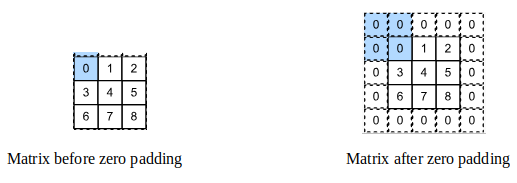
\includegraphics[width=0.8\linewidth]{img/zero_padding} 

}

\caption{Matrix showing zero padding.}\label{fig:zero_pad}
\end{figure}

\textbf{Same Padding}: This padding strategy is similar to zero padding
when zeros are added to the edges of an image. However, a different
figure, say 1, could be added on the edges of an image, which would make
the padding strategy different from zero padding. This type of padding
is also called constant padding.

\textbf{Valid Padding}: valid padding occurs when no extra data is
placed at the borders of a matrix or image. Essentially, it is best
understood as the absence of padding.

\textbf{Reflection Padding}: This padding technique works by extracting
pixels from the border of an image and adding them to the same border in
reverse order. It is notable that this padding technique is sometimes
referred to as symmetric or edge padding.

\begin{figure}

{\centering 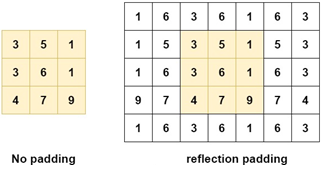
\includegraphics[width=0.8\linewidth]{img/reflection_padding} 

}

\caption{Matrix showing reflection padding.}\label{fig:reflect_pad}
\end{figure}

\textbf{Replication Padding}: replication padding is almost similar to
reflective padding only that rather than creating a reflection of the
pixels around the edges of a matrix or image it duplicates adjacent
values on the edges of the matrix or image. This padding strategy is
also called mirror padding.

\begin{figure}

{\centering 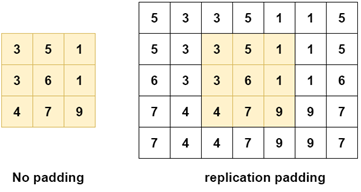
\includegraphics[width=0.8\linewidth]{img/replication_padding} 

}

\caption{Matrix showing replication padding.}\label{fig:rep_pad}
\end{figure}

\textbf{Circular Padding}: Wraps the image values on one side around to
the other side to provide the the matrix with additional data that is
required before a filter is applied. It is like data from the edges is
extracted and placed in the opposite side of the matrix

\begin{figure}

{\centering 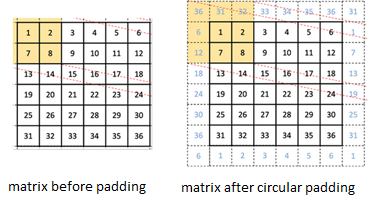
\includegraphics[width=0.8\linewidth]{img/cricular_padding} 

}

\caption{Matrix showing circular padding.}\label{fig:circ_pad}
\end{figure}

\textbf{Sequence Padding}: is a type of padding strategy commonly
applied to sequential or time series data. This padding technique is
thoroughly documented by Rio et al., (2020) and can be divided into
truncation padding, post-padding and pre-padding. Truncation padding
occurs when items in an array are trimmed to have the same length as an
array with the least length. Another padding strategy under sequence
padding is post-padding and occurs when a chosen value (usually zero) is
added at the end of short array items to make all short arrays equal to
the longest array. Pre-padding is the opposite of post-padding and
occurs when a chosen value (usually zero) is added at the beginning of
shorter arrays in a bid to make them equal to the longest array. This
type of padding could also be called causal padding.

\begin{figure}

{\centering 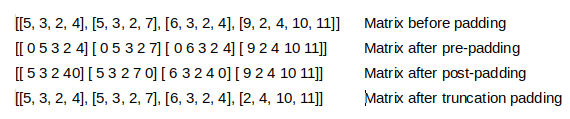
\includegraphics[width=0.8\linewidth]{img/sequence_padding} 

}

\caption{Matrix showing sequence padding.}\label{fig:seq_pad}
\end{figure}

~~~~~~~An array of studies have been published either introducing new
padding strategies or applying the already existing padding techniques
on different problems. For example, Nguyen et al., (2021) discusses
padding strategies such as partial convolution padding, mean
interpolation padding, and mean reflection padding. It is important to
note that while the authors discuss the aforementioned padding
strategies, the strategies are not the focal point of their publication.
It is because the authors also discuss distribution padding and conduct
an experiment on it. Eventually, the authors show that distribution
padding performs better than zero padding in image classification
problems. In a different publication, Ning et al., (2023) introduced the
idea of learning-based padding arguing that it performs better than the
traditional padding strategies. To be specific, the authors propose that
learning based paradigms could be used to calculate padding values from
data that is on the edge of images. The authors propose learning-based
padding by attention and learning-based padding by convolution as
methods that could be used to calculate padding values.

~~~~~~~Other authors have also investigated padding by developing new
padding strategies or examining how padding affects the training process
of neural networks. As evidence of this, Reddy and Reddy (2019)
investigated the effect of post-padding and pre-padding in Long
short-term memory (LSTM) neural networks and CNNs. The authors concluded
that post-padding and pre-padding improve the accuracy of LSTMs but not
CNNs because the architecture of CNNs forgets effects of time series
variations. Tang et al., (2019) also investigate the effect of invalid
and same padding using Pre-trained CNNs and concluded that padding with
a stride size set with a value close to the half of the image dimension
improves the performance. Another author, Cheng (2020), investigated the
effect of zero padding at the bottom of a text only and on all sides of
a text in natural language processing. Their study revealed that there
is no difference between applying padding at the bottom of a text and on
all sides of a text.

~~~~~~~Another publication investigating padding and how it relates to
convolution neural networks is from Alrasheedi et al., (2023). The
authors acknowledge that padding has been investigated shallowly. It is
then, that they propose a padding technique that learns from shifts in
hyper parameters of a CNN before adjusting padding effectively. Finally,
Alrasheedi et al., (2023) introduce a padding module providing evidence
that it performs better 1.49\% and 0.44\% more better in classification
accuracy than the zero padding when tested on the VGG16 and ResNet50.
Clearly a considerable number of publications investigating how padding
affects convolution neural networks have been made. Regardless, the
number of publications that investigate how padding affects CNNs in
computer vision still remain low. This owes to the fact that only one
study has been made investigating how padding affects CNNs has been
made. Moreover, no study has been found investigating the effect of
padding on CNNs with respect to facial recognition has been found. This
is a clear indicator that this proposed study will add value to the
already existing literature in facial recognition.

\subsection{Facial Recognition
Datasets}\label{facial-recognition-datasets}

~~~~~~~An array of studies have been conducted on facial recognition
implying that there exist several datasets that could be used for facial
recognition. Ayad et al., (2023) conducted a study discussing twenty-one
different datasets that have been used for research in facial
recognition. This publication discusses main characteristics of each
dataset and should be the first stop shop for authors looking to examine
data sets used for facial recognition. Ortis and Becker (2013) also
discuss facial recognition data sets only that they focus on web scale
datasets. This owes to the fact that web scale datasets are created for
facial recognition in real time and on the web. Such datasets should
scale well and be ready to be used for tagging friends or finding
celebrities online. Clearly, there are a lot of data sets that could be
used for facial recognition. However, access to such datasets have been
limited due to the recent changes in laws regarding access and use of
personal identifiable information.

\subsubsection{Disguised Faces in The Wild
Dataset}\label{disguised-faces-in-the-wild-dataset}

~~~~~~~The disguised faces in the wild dataset contains 11,157 images
collected from 1,000 different people. This data set was collected from
the internet and was released in 2018 during the Disguised Faces in the
Wild Workshop at International Conference on Computer Vision and Pattern
Recognition (Singh et al., 2018). Critical to the discussion is the
reality that the disguised faces in the wild (DFW) was developed with an
aim of creating facial recognition models that are resistant to
disguises. This owes to the fact that Singh et al., (2018) acknowledge
that humans could artificially alter their faces with an aim of fooling
a facial recognition system. For instance, an individual could try and
fool a system by wearing a wig, wearing at artificial beard or putting
on heavy make up. It is important to note that a different dataset
called Disguised Faces in the Wild 2019 Dataset has been published and
should be confused for the dataset under discussion (Singh et al.,
2019). Clearly, this is an interesting subject of study that should be
investigated further using the dataset in question.

\subsubsection{VGGFACE}\label{vggface}

~~~~~~~VGG Face dataset is made up of 2.6 million images collected from
2,622 different people. This dataset comprises mostly of politicians,
actors, public figures and celebrities, which was made by extracting
male's and females' information from the Internet Movie Database and
ranked by popularity (Parkhi et al., 2015). Critical to the discussion
is the fact that this data set was examined by human annotators to
eliminate images that could introduce noise into the dataset. It is
important to highlight that this dataset has been used and cited by
authors widely. For example, Ibrahem and Abdulameer (2023) examine a
pretrained model that was created from this dataset to discuss a model
aimed at solving the age problem associated with facial recognition.
While the number of publications that have used this dataset remains
low, the number of publications that have used the pretrained model from
this dataset is high. This explains why the researcher will be using a
pretrained model from this dataset for this study.

\subsubsection{KomNET Face Dataset}\label{komnet-face-dataset}

~~~~~~~The KomNET face dataset comprises of 39,600 images but the number
of people whose faces were collected from is not stated in the
publication associated with the dataset (Astawa et al., 2020). It is
however crucial to note that the dataset was collected from social
media, collected using a digital camera, and a smartphone. As already
mentioned, some of the challenges associated with facial recognition
include occlusion and the lighting conditions in images. That said, it
is important to highlight the dataset in question is limited by the fact
that different lighting conditions were not taken into consideration
while collecting the images. Moreover, the number of images collected
was 1,200 images but they were subjected to augmentation to make them
39,600. Specifically, the images were subjected to augmentation
techniques such as average blur, emboss, flip, gamma contrast, gaussian
blur, histogram equalization, rotate, hue and saturation, sharpen, and
sigmoid contrast (Astawa et al., 2020).

\subsection{Facial Recognition
Architectures}\label{facial-recognition-architectures}

~~~~~~~Apparently, there have been multiple studies on facial
recognition implying there are multiples solutions to the problem of
facial recognition. To add insult to injury, some authors have conducted
reviews on some of the existing architectures on facial recognition. The
term architecture here refers to a deep learning model that could be
used to match or a recognize a face belonging to a particular person. An
example of an author that has conducted review on facial recognition
architectures is sun and Redei (2022). Specifically, the authors in
question discuss architectures such as FaceNet, DeepFace, DeepID-Net,
and Local binary patterns architectures. Gupta (2017) also reviewed some
of the existing architectures in facial recognition. In particular, the
author discusses architectures like WebFace, DeepFace, VGG Net, FaceNet,
and DeepId. Critical to the discussion is that fact that the number of
existing architectures could be more than 30 implying that discussing
all these architectures would be daunting. It follows that this paper
will only discuss selected architectures in order to stick to the scope
of the paper.

\subsubsection{Google FaceNet}\label{google-facenet}

~~~~~~~Google FaceNet, or popularly known as FaceNet, is a facial
recognition architecture that was developed by researchers at Google.
This architecture relies on an earlier architecture called Inception
Network, which generates convolution and concatenates the revolutions to
improve the efficiency of the architecture. While discussing Inception
Network would be an interesting subject, going into the details of it is
beyond the scope of this paper. Now, back to google net, the
architecture relies on a technique called the triplet loss function,
which calculates the distance (almost similar to the Euclidian distance)
between three images and returns a positive value when a match is found
(Schroff et al., 2015). Vital to the debate is the truth that this
architecture has been testes on face datasets called the YouTube Face
dataset and the Labelled Faces in the Wild dataset. Further, the
architecture recorded an accuracy of 95.12\% on the YouTube Face dataset
and recorded an accuracy of 99.63\% on the Labelled Faces in the Wild
dataset (Sun and Redei, 2022). It should be noted however that FaceNet
requires high performing computers in order to train the architecture on
a new dataset.

\subsubsection{DeepFace}\label{deepface}

~~~~~~~DeepFace was also produced by a giant company in technology.
Specifically, Meta. Critical to the discussion is the fact Taigman et
al., (2014) published the results from the study that produced DeepFace.
It is important to note that the researchers introduced an idea of 3D
modelling based on face fiducial points, which in turn is used to align
faces. Simply put, the facial alignment methodology proposed by Taigman
et al., (2014) can transform an image shown in figure 2.6 (a) to an
image shown in figure 2.6 (b). Resulting images from facial alignment
are then subjected to a deep convolution neural network architecture
that is thoroughly documented by Taigman et al., (2014). Vital to the
discussion is the fact that the DeepFace architecture was tested on the
Labelled Faces in the Wild dataset, and the YouTube Faces dataset. It
follows that this architecture achieved an accuracy of 97.5\% in the
Labelled Faces in the Wild dataset and a 91.4\% accuracy on the YouTube
Faces dataset.

\end{document}
